\section{Increasing Sensitivity through PCA}
So far in the analysis, all features have been given an equal weighting in the beginning of training,
But, as mentioned in section \ref{sec:MLHEP}, not all features contribute to an effective signal 
region. In section \ref{subsec:PCA}, I explained how through the use of \ac{PCA}, we are able to 
create a new set of features which can be ordered by amount of variance. In this way, we can reduce
the dimensionality of the data set, while at the same time preserving most of the variance. Inn this 
section I will present the results of training on a data set which has gone through such a \ac{PCA}.
\\
In this analysis I performed a \ac{PCA} on the data set, and demanded that $99.99\%$ of the variance 
should be preserved. In doing so, 5 features were removed. 
\subsection{NN and PCA}
\begin{figure}
    \makebox[\linewidth][c]{%
    \centering
    \begin{subfigure}{.65\textwidth}
        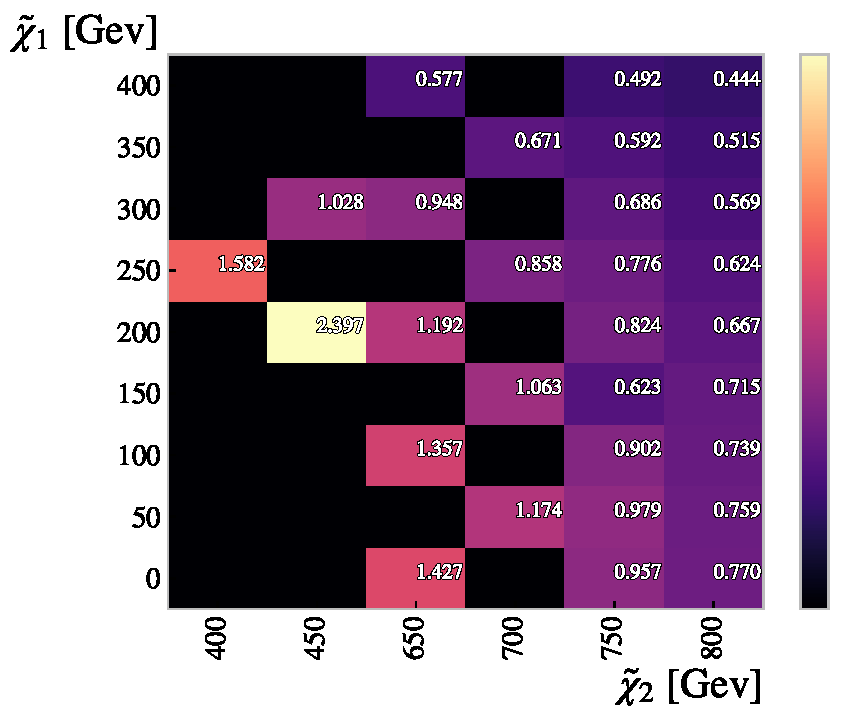
\includegraphics[width=\textwidth]{Figures/MLResults/NN/SUSY/Grid/NNPCAGridSig.pdf}
    \end{subfigure}
    }
    \caption{A grid displaying the achieved significance on the original signal set, using the signal region 
    created by the \ac{NN} network. A \ac{PCA} analysis has been applied to the data being utilized in this result.}
    \label{fig:NNPCAGridSig}
\end{figure}

\begin{figure}
    \makebox[\linewidth][c]{%
    \centering
    \begin{subfigure}{.65\textwidth}
        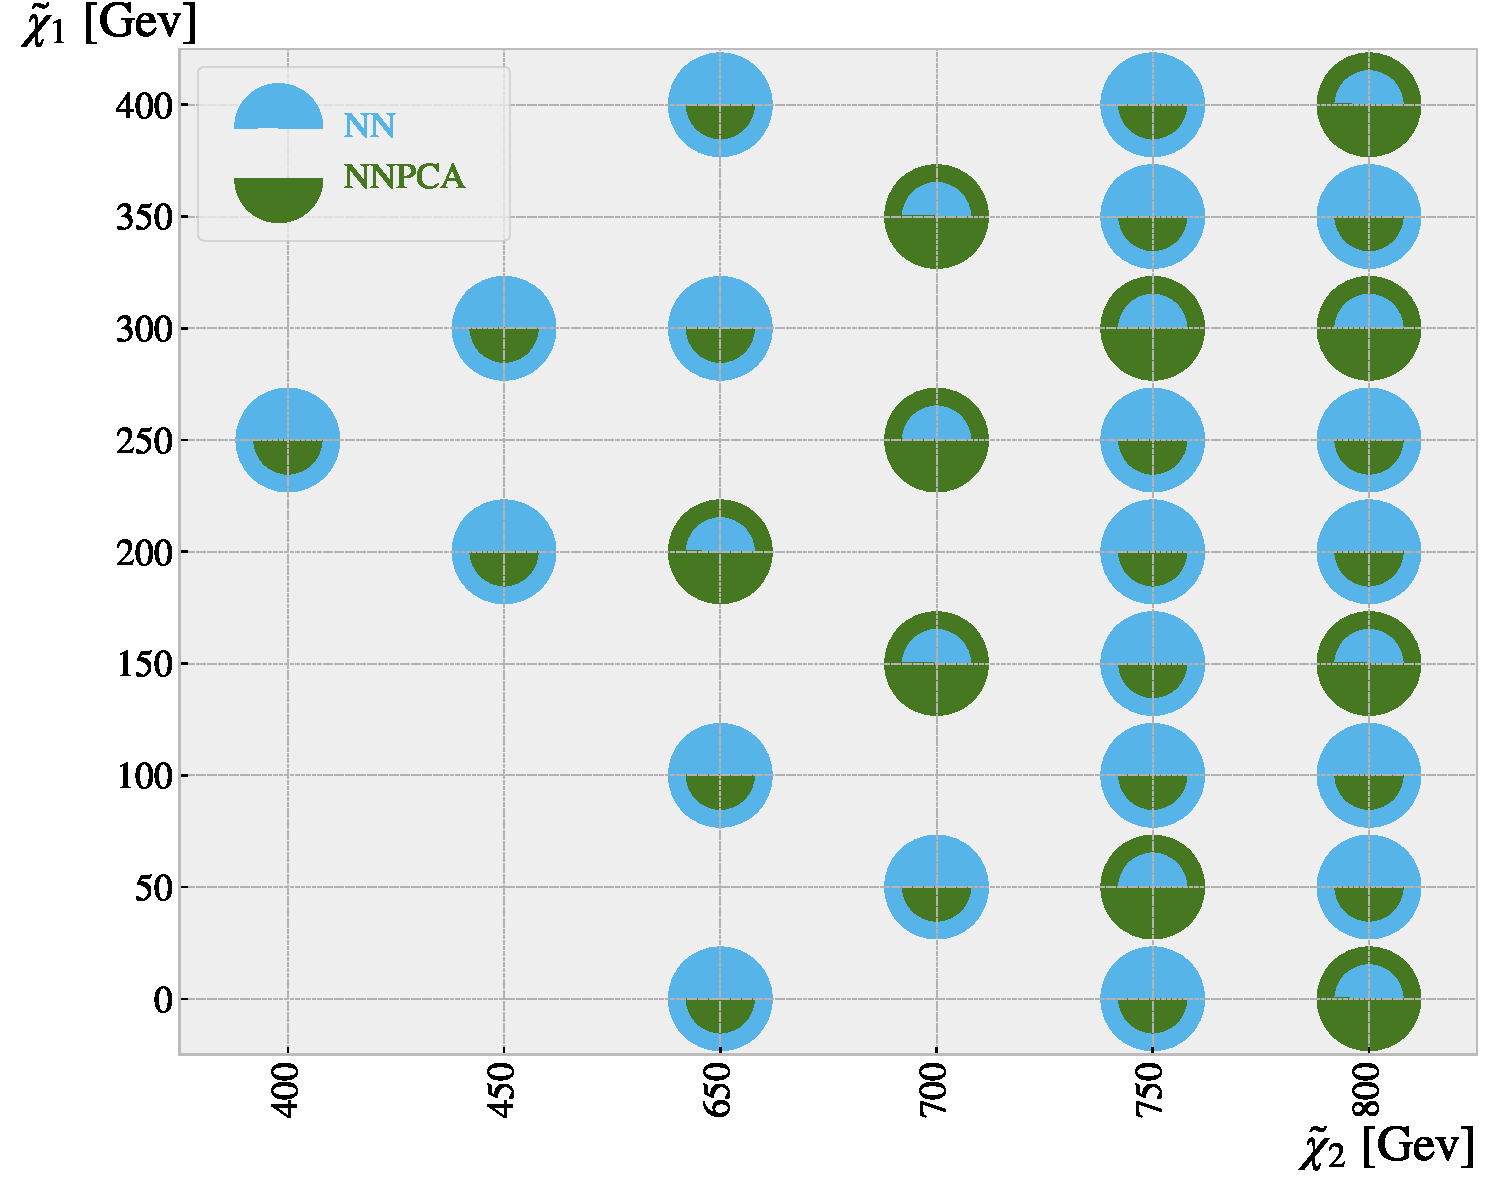
\includegraphics[width=\textwidth]{Figures/MLResults/NN/SUSY/Comparison/NNPCANetworkComp.pdf}
    \end{subfigure}
    }
    \caption{A grid displaying the achieved significance on the original signal set, using the signal region 
    created by the \ac{NN} network. A \ac{PCA} analysis has been applied to the data being utilized in this result.}
    \label{fig:NNPCAComp}
\end{figure}

\subsection{MaxOut Network and PCA}
\begin{figure}
    \makebox[\linewidth][c]{%
    \centering
    \begin{subfigure}{.65\textwidth}
        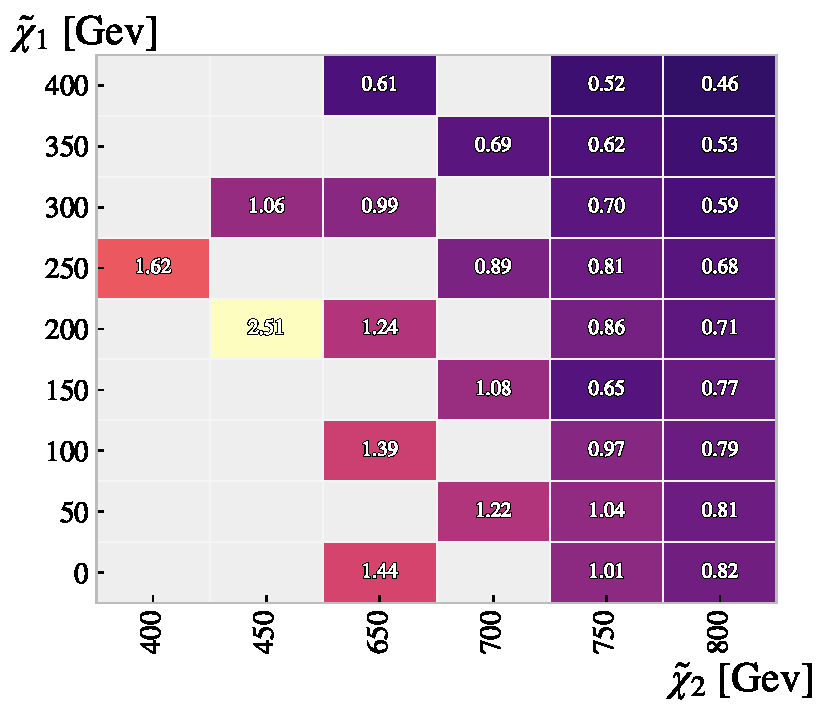
\includegraphics[width=\textwidth]{Figures/MLResults/NN/SUSY/Grid/MaxOutPCAGridSig.pdf}
    \end{subfigure}
    }
    \caption{A grid displaying the achieved significance on the original signal set, using the signal region 
    created by the \emph{MaxOut} network. A \ac{PCA} analysis has been applied to the data being utilized in this result.}
    \label{fig:MaxOutPCAGridSig}
\end{figure}
\begin{figure}
    \makebox[\linewidth][c]{%
    \centering
    \begin{subfigure}{.65\textwidth}
        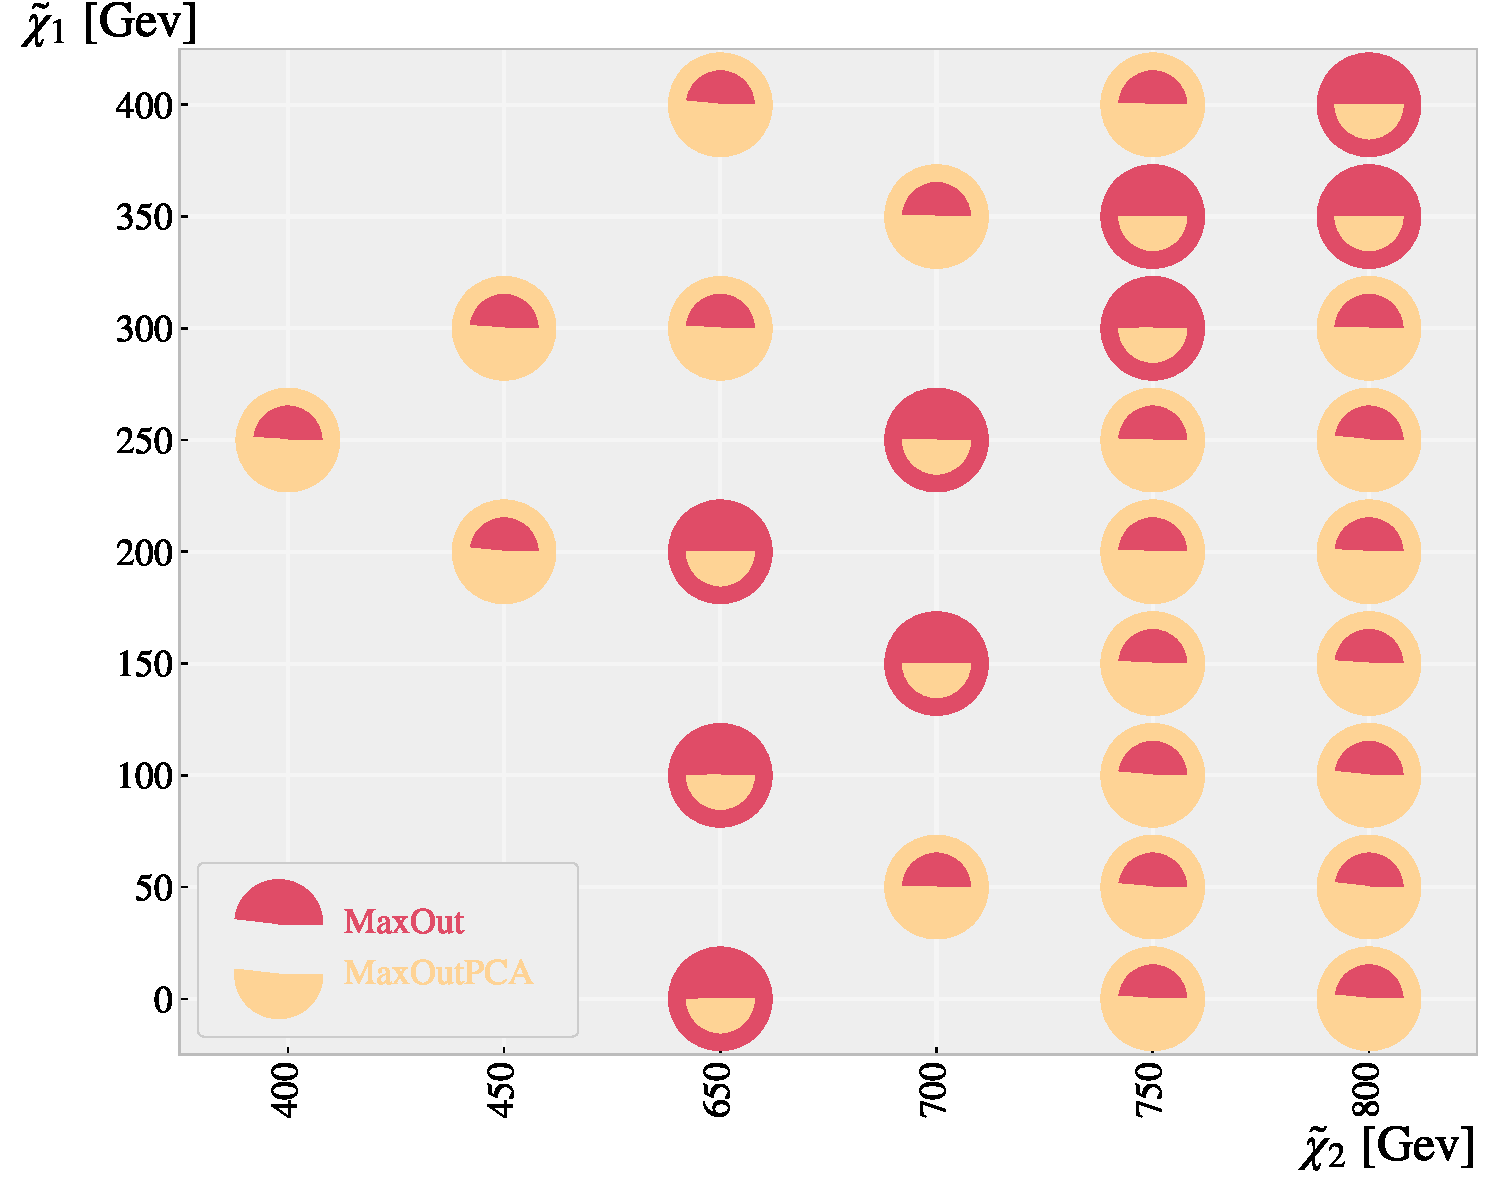
\includegraphics[width=\textwidth]{Figures/MLResults/NN/SUSY/Comparison/MaxOutPCANetworkComp.pdf}
    \end{subfigure}
    }
    \caption{A grid displaying the achieved significance on the original signal set, using the signal region 
    created by the \ac{NN} network. A \ac{PCA} analysis has been applied to the data being utilized in this result.}
    \label{fig:MaxOutPCAComp}
\end{figure}
\subsection{PNN and PCA}
\begin{figure}
    \makebox[\linewidth][c]{%
    \centering
    \begin{subfigure}{.65\textwidth}
        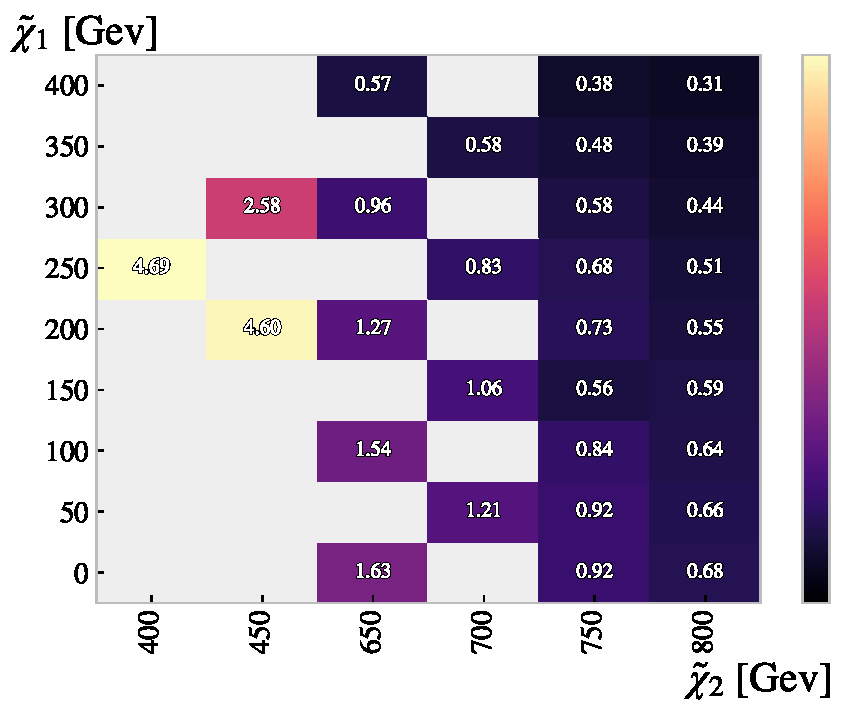
\includegraphics[width=\textwidth]{Figures/MLResults/NN/SUSY/Grid/PNNPCAGridSig.pdf}
    \end{subfigure}
    }
    \caption{A grid displaying the achieved significance on the original signal set, using the signal region 
    created by the \ac{PNN} network. A \ac{PCA} analysis has been applied to the data being utilized in this result.}
    \label{fig:PNNPCAGridSig}
\end{figure}
\begin{figure}
    \makebox[\linewidth][c]{%
    \centering
    \begin{subfigure}{.65\textwidth}
        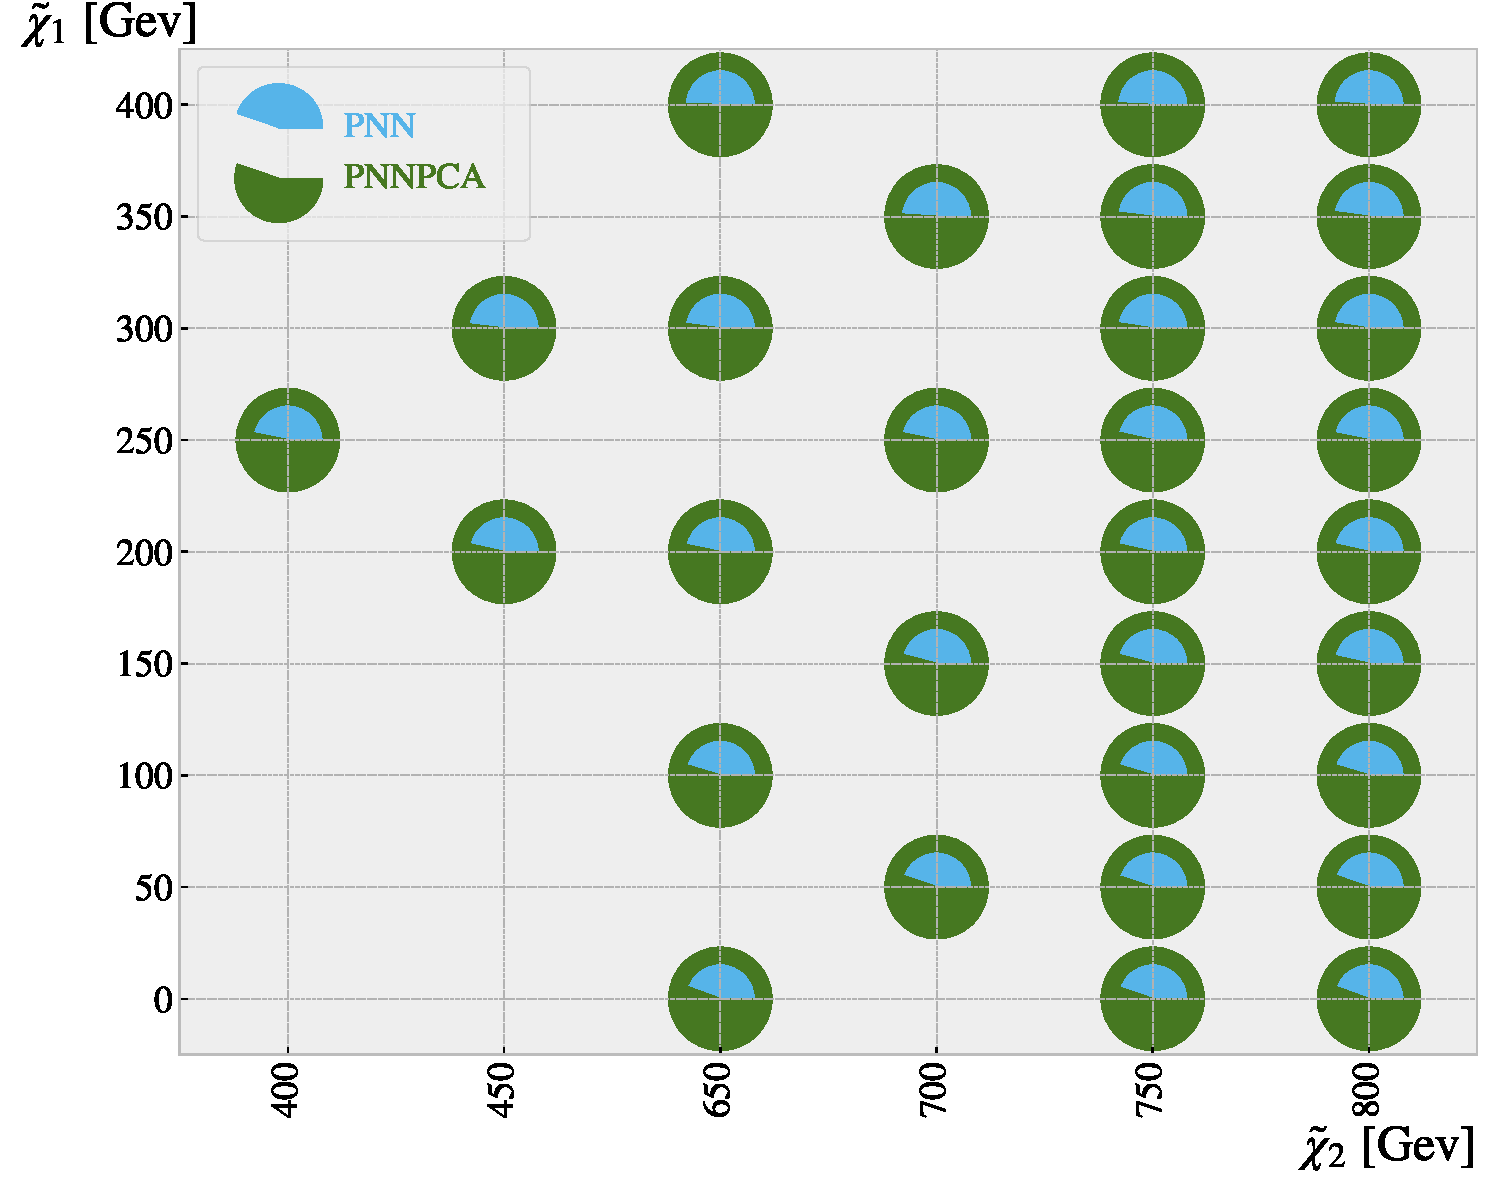
\includegraphics[width=\textwidth]{Figures/MLResults/NN/SUSY/Comparison/PNNPCANetworkComp.pdf}
    \end{subfigure}
    }
    \caption{A grid displaying the achieved significance on the original signal set, using the signal region 
    created by the \ac{NN} network. A \ac{PCA} analysis has been applied to the data being utilized in this result.}
    \label{fig:PNNPCAComp}
\end{figure}

\begin{figure}
    \makebox[\linewidth][c]{%
    \centering
    \begin{subfigure}{.65\textwidth}
        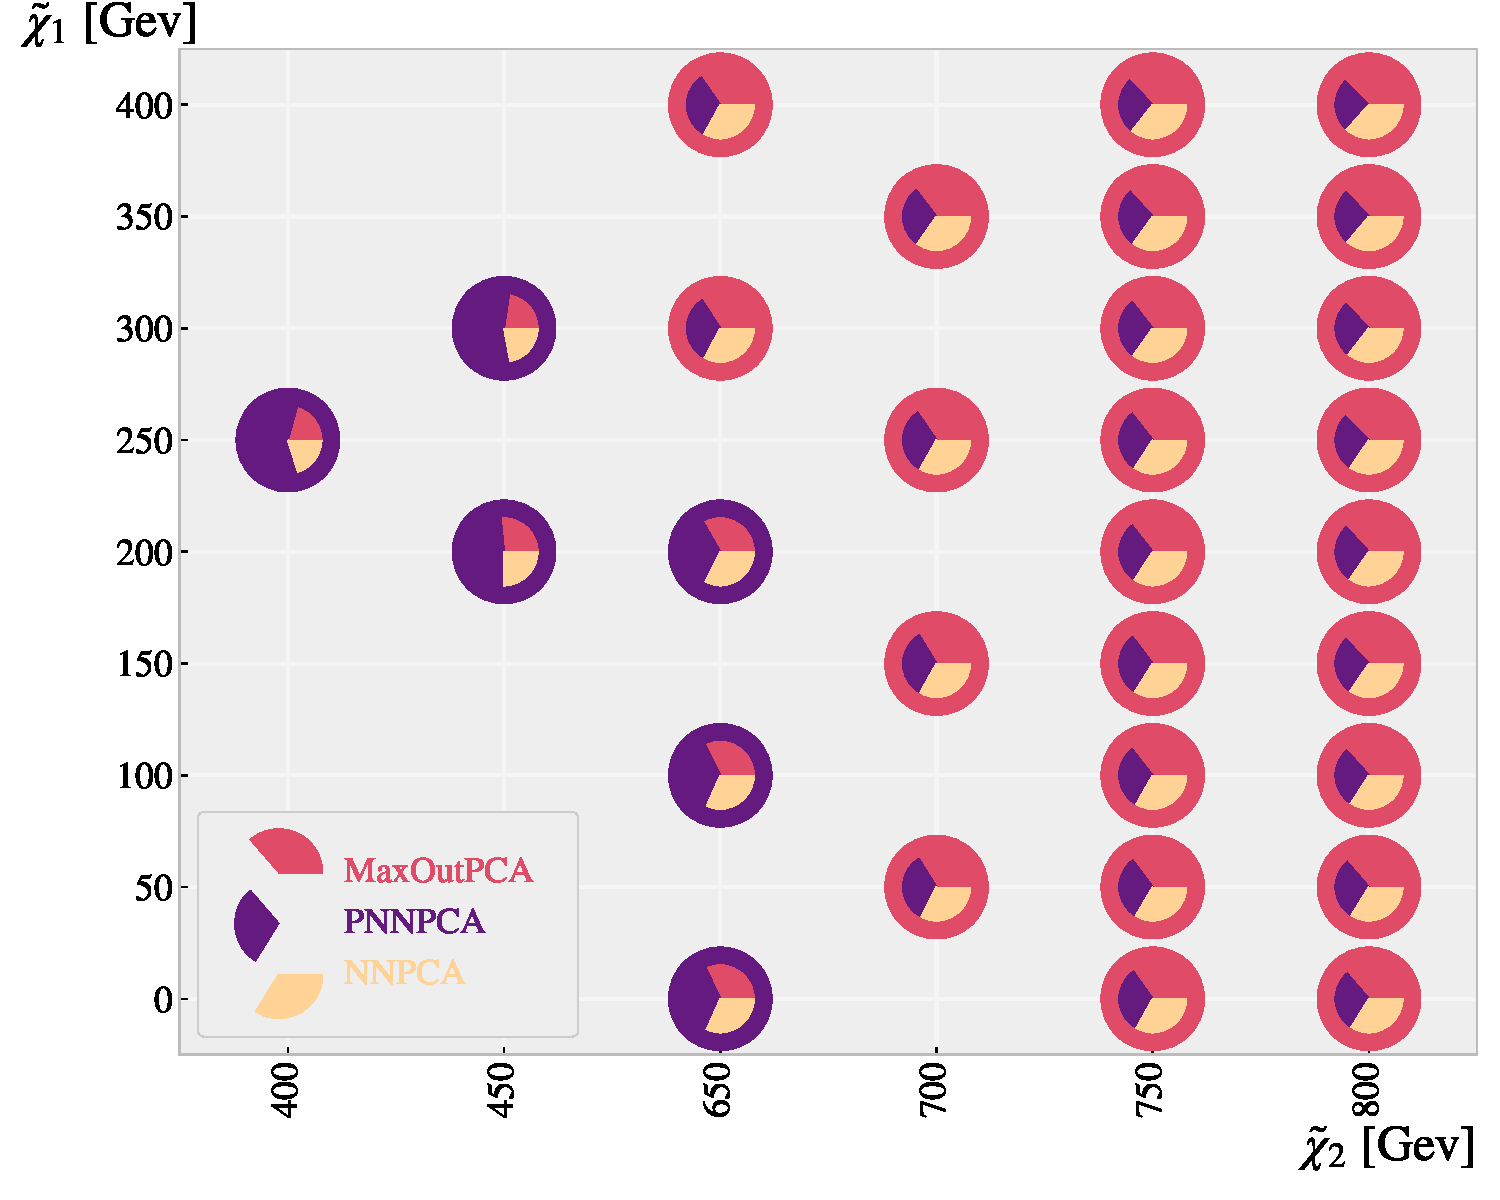
\includegraphics[width=\textwidth]{Figures/MLResults/NN/SUSY/Comparison/PCANetworkComp.pdf}
    \end{subfigure}
    }
    \caption{A grid displaying the achieved significance on the original signal set, using the signal region 
    created by the \ac{NN} network. A \ac{PCA} analysis has been applied to the data being utilized in this result.}
    \label{fig:PCAComp}
\end{figure}
